\section{What is this? And why should I use it?}
\label{sec:what_is_this_and_why_should_i_use_it}

Among the needs of the persons involved in higher education, we identified
the following:
%
\begin{description}
	\item[for students:] when studying, have a clear idea of how courses
		connect to each other from a contents-wise perspective, and
		of why it is important to memorize and understand what it is
		being asked to study (e.g., why shall I understand what is
		the geometrical interpretation of eigenvalues?);
	\item[for teachers:] when modifying the contents of the own courses,
		have a holistic view on the effects of these contents
		modifications on the program (e.g., if I won't teach this
		concept anymore in my course, how will this affect the
		following courses?);
	\item[for program boards:] when modifying the structure of a
		program, have instruments that help steering discussions and
		taking decisions based on evidence instead of opinions
		(e.g., why shall this course be taught before that other
		one?);
	\item[for administrators:] when inspecting and assessing the program
		quality, have instruments that are quantitative oriented,
		explainable, and communicable, so to ease discussions and
		reporting.
\end{description}

\begin{centering}
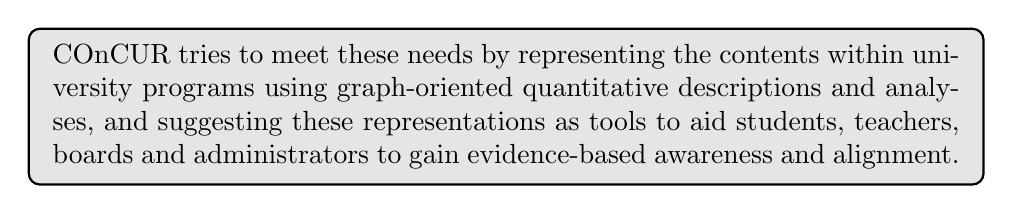
\begin{tikzpicture}
\node [minimum width = \textwidth, rounded corners, draw, thick, fill =
	black!10!white, align = justify, text width = 0.95\textwidth, inner
	sep = 0.2cm]
{COnCUR tries to meet these needs by representing the contents within
	university programs using graph-oriented quantitative descriptions
	and analyses, and suggesting these representations as tools to aid
	students, teachers, boards and administrators to gain evidence-based
	awareness and alignment.};
\end{tikzpicture}
\end{centering}

The approach is the following: 
\begin{enumerate}
	\item consider courses and programs as opportune flows and
		transformations of prerequisite contents-wise knowledge
		(expressed in terms of prerequisite \acp{KC}) into developed
		contents-wise knowledge (expressed in terms of developed
		\acp{KC}. See Section~\ref{sec:lexicon} for an explanation
		of all the various terms); 
	\item analyze and visualize the structure of a program (or a part of
		it) in terms of these \ac{KC} development flows;
	\item connect these flows to the \acp{TLA}, \acp{ILO} and \acp{PLO}
		of the various courses and the whole program;
	\item increase the awareness of the stakeholders by visualizing and
		analyzing these connections and flows in self-explanatory
		ways.
\end{enumerate}

\begin{example}
	%
	To exemplify this process, assume that the contents of the
	fictitious ``\emph{Course X}'' can be expressed in terms of which
	prerequisite \acp{KC} are required by the students plus which
	\acp{KC} are developed in the course itself. E.g., let the
	prerequisites and developed \acp{KC} be:
	%
	\begin{itemize}
		\item prerequisites: ``\emph{vector spaces}'',
			``\emph{linearity}'', and ``\emph{matrices-vectors
			multiplication}'';
		\item developed: ``\emph{eigenvalues}'',
			``\emph{characteristic polynomials}'',
			``\emph{computation of Jordan forms}''.
	\end{itemize}
	%
	Ideally, and as an example, the teacher knows that the developed
	\acp{KC} are reached by building on the prerequisite ones as
	summarized in Figure~\ref{fig:KCM}. I.e., in the ideal case,
	%
	\begin{itemize}
		\item to be able to learn about \emph{eigenvalues}, students
			should have reached learning level (using Bloom's
			taxonomy~\cite{bloom1956taxonomy} as an illustrative
			example) two (understand) for both prerequisites
			\emph{vector spaces} and \emph{linearity} by the
			time that \ac{KC} is taught;
		\item to be able to learn about \emph{characteristic
			polynomials}, they should have reached learning
			level two for \emph{matrices and vectors
			multiplication}, and have reached learning level one
			(remember) about the developed \ac{KC}
			\emph{eigenvalues} while studying \emph{Course X};
		\item to be able to learn about \emph{computation of Jordan
			forms}, they should have reached learning level one
			for the prerequisite \emph{linearity} and level two
			for the developed \emph{eigenvalues} and
			\emph{characteristic polynomials}.
	\end{itemize}
	%
	\begin{figure}[!htbp]
		\centering
		\begin{tikzpicture}
[
	Concept/.style	= {font = \scriptsize, align = center, anchor = base, minimum height = 1cm},
	row sep			= {1cm,between origins},
	column sep		= {1.9cm,between origins},
	column 1/.style	= {column sep = 1cm, nodes = {fill = black!00!white}, },
]

	\matrix (M)
	[
		matrix of nodes,
		nodes					= {font = \footnotesize, inner sep = 0cm, text height = 0.3cm, text width = 0.65cm, align = center, anchor = base},
		nodes in empty cells	= true,
	]
	{
		45\%  & 2 & 2 &   &   &   &   & 3 \\
		20\%  &   &   & 2 & 1 &   &   & 2 \\
		35\%  &   & 1 &   & 2 & 2 &   & 3 \\
	};

	\node (p0) [Concept, above = 0.5cm of M-1-1, minimum width = 1.7cm] {teaching \\ \phantom{g} time \phantom{g}};
	\node (p1) [Concept, above = 0.5cm of M-1-2] {vector \\ spaces};
	\node (p2) [Concept, above = 0.5cm of M-1-3] {linearity};
	\node (p3) [Concept, above = 0.5cm of M-1-4] {matrix-vector \\ multiplication};
	%
	\node (p4) [Concept, above = 0.5cm of M-1-5] {eigenvalues};
	\node (p5) [Concept, above = 0.5cm of M-1-6] {characteristic \\ polynomials};
	\node (p6) [Concept, above = 0.5cm of M-1-7] {compute \\ \phantom{g} Jordan forms \phantom{g}};
	%
	\node (p7) [Concept, above = 0.5cm of M-1-8, minimum width = 1.7cm] {intended \\ final knowledge \\ level};
	%
	\node (c1) [Concept, left = 0.5cm of M-1-1] {eigenvalues};
	\node (c2) [Concept, left = 0.5cm of M-2-1] {characteristic \\ polynomials};
	\node (c3) [Concept, left = 0.5cm of M-3-1] {compute \\ Jordan forms};

	\node (auxA) [coordinate, above = 0.5cm of p1.west, xshift = +0.1cm] {};
	\node (auxB) [coordinate, above = 0.5cm of p3.east, xshift = -0.1cm] {};
	\node (auxC) [coordinate, above = 0.5cm of p4.west, xshift = +0.1cm] {};
	\node (auxD) [coordinate, above = 0.5cm of p6.east, xshift = -0.1cm] {};
	%
	\draw [decorate, decoration = brace, draw = black!50!white] (auxA) -- (auxB) node [above, pos = 0.5, font = \scriptsize, text = black!50!white] {prerequisite concepts};
	%
	\draw [decorate, decoration = brace, draw = black!50!white] (auxC) -- (auxD) node [above, pos = 0.5, font = \scriptsize, text = black!50!white] {developed concepts};

	% auxiliary nodes to draw the matrix
	\node (MM11) [coordinate] at (c1.north east) {};
	\node (MM21) [coordinate] at (c3.south east) {};
	\node (MM12) [coordinate] at ($(p0.north east)!(c1.north east)!(p0.south east)$) {};
	\node (MM22) [coordinate] at ($(p0.north east)!(c3.south east)!(p0.south east)$) {};
	\node (MM13) [coordinate] at ($(p6.north east)!(c1.north east)!(p6.south east)$) {};
	\node (MM23) [coordinate] at ($(p6.north east)!(c3.south east)!(p6.south east)$) {};

	\draw [solid] (MM11) -- (MM21);
	\draw [solid] (MM21) -- (MM23);
	\draw [solid] (MM23) -- (MM13);
	\draw [solid] (MM13) -- (MM11);
	\draw [solid] (MM12) -- (MM22);

\end{tikzpicture}


		\caption{Tabular representation of how \emph{Course X}'s
		developed concepts are ideally reached by building on its
		prerequisites. This matrix is known as a \acf{KCM} in this
		manual.}
		\label{fig:KCM}
	\end{figure}
	%
	The \ac{KCM} in Figure~\ref{fig:KCM} can be converted into its graph
	representation defined in Figure~\ref{fig:KCG}.
	%
	\begin{figure}[!htbp]
		\centering
		\begin{tikzpicture}
[
	ILO/.style	= {circle, draw = black!50!white, fill = black!10!white, minimum size = 0.7cm, inner sep = 0cm, font = \scriptsize},
	pre/.style	= {ILO, draw = black, fill = white},
	comment/.style	= {font = \footnotesize},
	node distance = 0.8cm and 0.8cm,
	every path/.style = {-latex, thick, shorten < = 0.1cm, shorten > = 0.1cm},
]

	\node (pre1) [pre] {};
	\node (pre2) [pre, below = of pre1] {};
	\node (pre3) [pre, below = of pre2] {};
	%
	\node (ILO1) [ILO, right = 2cm of pre1] {45\%};
	\node (ILO2) [ILO, below = of ILO1] {20\%};
	\node (ILO3) [ILO, below = of ILO2] {35\%};
	%
	\node (aux1) [coordinate, right = 4cm of ILO1] {};
	\node (aux2) [coordinate, right = 4cm of ILO2] {};
	\node (aux3) [coordinate, right = 4cm of ILO3] {};

	\node [comment, above left = 0cm of pre1] {vector spaces};
	\node [comment, above left = 0cm of pre2] {linearity};
	\node [comment, above left = 0cm of pre3] {matrix-vector multiplications};
	%
	\node [comment, above right = 0cm of ILO1] {eigenvalues};
	\node [comment, above right = 0cm of ILO2] {characteristic polynomials};
	\node [comment, above right = 0cm of ILO3] {compute Jordan forms};

	\draw (pre1) -- (ILO1) node [pos = 0.25, above] {2};
	\draw (pre2) -- (ILO1) node [pos = 0.25, above] {2};
	\draw (pre2) -- (ILO3) node [pos = 0.25, above] {1};
	\draw (pre3) -- (ILO2) node [pos = 0.25, below] {2};

	\draw (ILO1) -- (ILO2) node [pos = 0.5, right] {1};
	\draw [out = 235, in = 125] (ILO1) to node [pos = 0.35, left] {2} (ILO3);
	\draw (ILO2) -- (ILO3) node [pos = 0.5, right] {2};

	\draw (ILO1) -- (aux1) node [pos = 1.0, right] {3};
	\draw (ILO2) -- (aux2) node [pos = 1.0, right] {2};
	\draw (ILO3) -- (aux3) node [pos = 1.0, right] {3};


\end{tikzpicture}

		\caption{Graphical representation of the \acf{KCM} in
		Figure~\ref{fig:KCM}, which is known as a \acf{KCG} in this
		manual.}
		\label{fig:KCG}
	\end{figure}
	%
	Within a program, the \acp{KC} developed in some courses may be
	prerequisites for other courses. This means that one can join the
	various individual \acp{KCM} and \acp{KCG} into a program-wide
	representation. This operation produces a directed graph
	representing the various ``\emph{\acp{KC} learning flows}'' that
	students ideally follow during their studies. 
	%
\label{exa:KCM}
\end{example}

\ac{KCG} representations can help meeting the stakeholders' needs listed at
the beginning as follows:
%
\begin{description}
	\item[for teachers:] changing the contents of a course means
		changing the learning flows in the \ac{KCG}. With the
		proposed software, one can check if modifying a course
		(here: the \ac{KCM}) is going to lead to broken, redundant
		or non-ideal pedagogical paths in the \ac{KCG};
	\item[for program boards:] the same software may be used to manage
		the discussions during board meetings, and act as a digital
		canvas where the meaningfulness of different program changes
		can be evaluated. This may help taking an evidence-based
		approach to designing and modifying programs;
	\item[for students:] the software may be used by students to get
		intuitions about the purpose of studying specific \acp{KC},
		understanding the effect of having forgotten parts of the
		program as well as how central each part is within the
		program flow. The software may thus help students perform
		self-assessment and monitoring, and help gaining holistic
		viewpoints on the expected learning process;
	\item[for quality assurance personnel:] the software may be used
		also by quality assurance to perform automatic assessments
		of structural properties of the programs. We envision to use
		these representations also to help performing comparisons of
		different programs at different institutions; these features
		are not yet implemented, however.
\end{description}

\subsection{What if I just want to analyse a single course?}

The software may be used by a teacher or set of teachers also in the context
of a \emph{single course}. In other words, in the following one may build up
a \ac{KCM} for each \emph{individual class} instead of for each
\emph{individual course}. This means that this software may be used as it is
also for planning, visualizing, assessing and discussing the detailed
contents of a course, instead of a program or part of it.
